
\section{Introduction}

This report will delve into the backward induction method of Dynamic Programming (DP) that applied to a stochastic finite-horizon dynamic decision problem. Here, we will focus on solving a specific variant of the knapsack problem, by calculating the optimal policy with some problem setting. To prove its effectiveness, we also implemented a deterministic method to find out the best solution. With the same random item list, we can testify to the effectiveness of our method. 

For the structure of the report, we will first introduce the mathematical {tbc} of the method, by doing this, we can come out with Hypotheses for our expected result. After explaining the implementation of the code, we will do experiments.
\section{Problem Analysis}
%Explain the problem
%At first, you should explain what the problem is that you are going to solve. What are your assumptions and why do they make sense or where do they deviate from reality.
\begin{table}
    \centering
    \caption{Parameter applying to both EAs}
    \label{tab:my_label}
    \begin{tabular}{@{}cc@{}}
     \hline %\midrule
        Parameter & Value \\ \hline
        Item size & 1 - 10 \\
        Time horizon & 10 \\
        knapsack capability & 10 \\
        Item weight probability & 0.1 \\
        Experiment runs & 1000\% \\\hline
    \end{tabular}
\end{table}

In the knapstack problem, the item weights is unknown upfront, thus, in each time step, the player needs to decide whether to take the item, based on the single weight and the remaining capability of the knapsack, who's total size is fixed at the beginning. 
Specifically, the sizes and other parameters are present in table \ref{tab:my_label}.

To formulate this problem, we set each presence of the action as one time step $t \in T:{1,2,...,10}$. The action set for each time step only depends on the time and state $x$, where $x \in X = {0, 1, 2, ...,10}$, representing the leftover capacity of the knapsack. Since one mustn't take an item larger than capacity, we have the equation \ref{eqo:1} of the action set. 
\begin{equation}
\label{eqo:1}
A_x = \left\{
\begin{aligned}
    &\{0, 1\} & if\ x - weight_t >0 \\
    &\{0\} & else
\end{aligned}
\right.
\end{equation}

\subsection{Deterministic value and transition}
For a Deterministic problem, the transition of state only depends on the cost at the time t. Namely, the action $a^t_x$ has a cost and a reward, where the cost of action, $c^t_a = a^t_x * weight_t$ equal to the item's weight if $a^t_x = 1$, while the reward $r^t_a$ is also 1 or 0, which would be added inductively to find the maximal value $v^t_x$ and the optimal policy for the action. Thus, for the value and transition function, we have:
\begin{equation}
    v_t(x) = r^t_a + V_{t+1}(x-c^t_a),t\in T, x \in X, a\in A_x
\end{equation}
\begin{equation}
    T_t(x,a) = x - c^t_a, t\in T, x \in X, a\in A_x
\end{equation}

\subsection{Stochastic value and transition}
Different from the deterministic problem, the transition at time t is stochastic, and the reward for an action is unknown. Therefore, to find the maximal value and optimal action at each state, we use the expected average of the foreseeing value $v_{t+1}$ times each transition probability, as follows:
\begin{equation}
    T(x,a) = x - c_t'*a, c_t'\in \{1,,,10\}, p_{c=c'} = 0.1
\end{equation}
\begin{equation}
    V_t(x) = \max_{a\in A_x}(1*a_x^t + \sum_{x' = T(x,a_x^t)} V_{t+1}(x')*p(x-c=x'))
\end{equation}
However, because of doing backward induction and the initial value for each state is zero, in the time t=10, the value of a state will only depend on the action, and $V_t+1(x)$ will introduce no diversity for any $weight_t<x$, thus, we define the policy $s$ as the minimal taken item size for each time t and state x, where $s_x \in {0,1,2,...,x}$, for the correctness, we will prove that in section \ref{sec:1.a}.

The expected average reward for such a $s$ is:
\begin{equation}
    \begin{aligned}
    reward(s)  
    & =1*p_{c\leq s} + 0 * p_{c > s}\\
    & =p*s
    \end{aligned}
\end{equation}
The new value function can be defined as:
\begin{equation}
\begin{aligned}
    V_t(x) = &\max_{s\in {0,1,2,...,x}}(reward(s) + \sum\limits_{i=0,x-c'=x'}^s V_{t+1}(x')*p(c=c'))\\
    =&\max_{s\in {0,1,2,...,x}}(s*p + \sum\limits_{i=0,x-c'=x'}^s V_{t+1}(x')*0.1)
\end{aligned}
\end{equation}
where $p(c=c')=0.1$ for all $c\in \{1,2,...,10\}$
\subsection{a) Correctness proof}
\label{sec:1.a}
As discussed in the last section, we take the maximal taken size $s$ as the optimal policy, thus, with backward induction, we can conclude that the expected reward would have a higher possibility to gain a better reward. To prove the policy correctness, it is equalient to prove that $V_t(x) \leq V_t(y), \forall x < y,t\in T$

Proof:
suppose at time $t$, the transition of states $x,\forall x < s$ and the optimal policy $s$ would be in three cases, then the resulting value for time $t+1$ would be

\begin{equation}
    V_{t}(x) = \left\{
    \begin{aligned}
    &V_{t+1}(x), if\ weight_t \ge x \\
    &\max (V_{t+1}(x), V_{t+1}(x-weight_t) + 1), else
\end{aligned}
\right.
\end{equation}
At the beginning, the value of each state is 0, the value only depends on the immediate rewards, namely, $V_t(x)=reward_t(x)$ at time $t=10$, and 
\begin{equation}
    reward_{t}(x) = \left\{
    \begin{aligned}
    & = reward_{t}(y) = 0 &if\ weight_t \ge y \\
    & = 0 < reward_t(y) = 1& if\ x < weight_t \leq y\\
    & = reward_t(y) = 1 & if\ weight_t < x
\end{aligned}
\right.
\end{equation}
For all $x<y$, It always holds that $reward_{t}(x)\leq reward_{t}(y)$, and thus $V_{10}(x) \leq V_{10}(y)$
 
While With $t<10$, the optimal value for a state x would be:
\begin{itemize}
    \item if $weight_t \ge y$:\\
    $$V_t(x) = V_{t+1}(x) \leq V_{t}(y) = V_{t+1}(y)$$
    \item if $x < weight_t \leq y$:\\
    $$\begin{aligned} V_t(x) &=V_{t+1}(x)\\ &\leq V_{t}(y) = \max(V_{t+1}(y), V_{t+1}(y-weight_t)+1)\end{aligned}$$
    \item if $weight_t \leq x$:\\
    $$\begin{aligned} & V_t(x) = \max(V_{t+1}(x), V_{t+1}(x-weight_t)+1),\\
    & V_{t}(y) = \max(V_{t+1}(y), V_{t+1}(y-weight_t)+1),\\
    & V_{t+1}(x-weight_t)<V_{t+1}(y-weight_t),\\
    & \rightarrow V_t(x) \leq V_t(y)
    \end{aligned} $$
\end{itemize}
 
Thus, for all $x<y$, any $t \in T$, it always holds that $V_t(x)<V_t(y)$

Now returning to the problem, it is also optimal to take item size smaller than s, because the remaining capacity would be smaller than the expected optimal, and therefore, a higher value than the optimal solution if take item of size s. 

\subsection{Hypotheses}
\begin{enumerate}[label=(\roman*)]
    \item\textbf{Hypothesis 1:} The optimal reward V at time 0 state 10 will be near the average reward of the experiments
    \item\textbf{Hypothesis 2:} Average reward smaller than the deterministic result, while the average remained weights of the optimal solution, would be at least 4 more according to the policy.
\end{enumerate}

\section{Methods}

%Describe your methods
%From your report, it should become clear what you did exactly and why this makes sense. In general, you can use as a guideline that a reader should be able to repeat your methods and is able to get to the same results. You can assume that your target audience would be any another student in the same study area. But this does not mean that you can leave out any parts up to be guessed / filled in by the reader. It is not required that your grandmother can understand it, however being able to explain her what you did is a good exercise that will come in handy whenever you plan to work in/for companies, where you will also oEen have to explain what you have done to persons lacking any mathema>cal/programming knowledge.
%For this specific assignment, this means that:
%-Copying the provided value function as given is not sufficient. Explain why it makes sense and don’t forget to add the base cases/boundary conditions.
%-Just sta>ng that you did a simula>on is not sufficient. Explain how this was done / what was exactly simulated and what was used from your solution in the first part.
\subsection{Algorithm Implementation}

As discussed above, the possible state set would be $X = {0,1,2,3,...,10}$, and time set $T = {1,2,3,...,10}$, thus, we implement a policy matrix with size $11 * 10$, while value set $V$ need to take account the beginning state, we add one more row $V_{11}$ all set to zero.

Since the problem starts as time 0 and state 10, the expected revenue would be $V_0[10] = 3.40634474$

For the test of the policy $Alpha$, we start with initializing a random weight list of size $|T|=10$, each between 1 and 10, then for each item, with an initial state of $x=10$, if $weight_t \leq Alpha_t[x]$, then do the transition $x=x-weight_t$, and the reward increase by one $v=v+1$. Else, move to the next item without any change. The final value at time 10 would be the optimal revenue.

The test will run 1000 times, and the average of the values should be close to the expected revenue of our policy, where we have hypothesis 1.

Additionally, there will also be the chance that the deterministic reward is higher using the optimal policy since we have an upper bound for the taken item weight that $s-weight_s \geq 0$, while in a deterministic method, the decision is only restricted by the state where $x-weight_t \geq 0$, and one can also decide not to take an item smaller than $s$, this introduce the difference. Therefore, if a different decision at some time is made and has an influence on the final revenue, this should also be shown in the leftover weight
Regarding that in the optimal policy, we have the difference $\min(x-s) = 0$ and $\max(x-s)=6$

To test its correctness, we also implement a backward induction method to find the deterministic best reward, and compare it 


\subsection{Experimental design and setup}

%Report your results
%You should report all (requested and/or relevant) results in a meaningful way. Report on the exact outcomes or provide plots, whatever makes the most sense in the situa>on. The goal should be that the reader gets presented all the insights that you want to show, in a clear way



\section{Results and Discussion}
%figures
\begin{figure*}[htbp]
    \centering
    \begin{subfigure}[htbp]{0.33\textwidth}
        \centering
        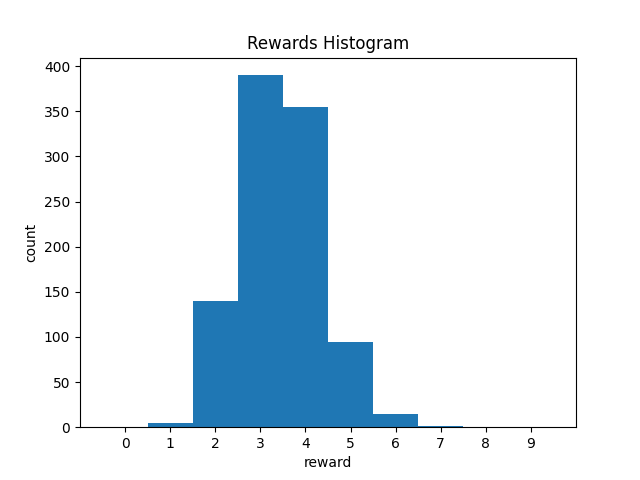
\includegraphics[width=\textwidth]{fig/asg1_reward_hist.png}
        \caption{rewards histogram over 1000 runs}
        \label{fig:fig_1}
    \end{subfigure}
    \hfill
    \begin{subfigure}[htbp]{0.33\textwidth}
        \centering
        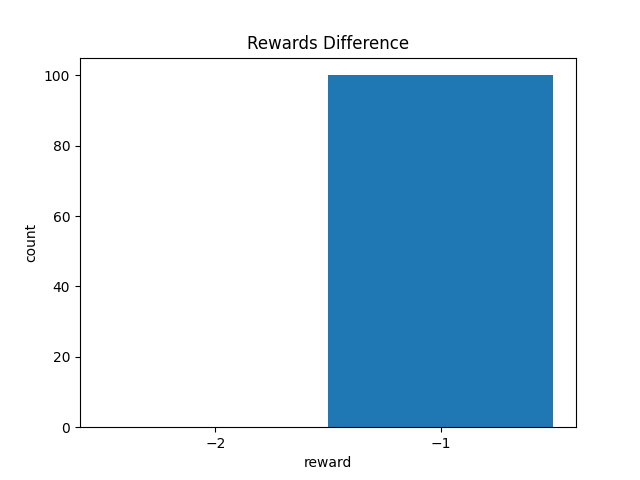
\includegraphics[width=\textwidth]{fig/asg1_reward_diff.png}
        \caption{correctness}
        \label{fig:fig_2}
    \end{subfigure}
    \hfill
    \begin{subfigure}[htbp]{0.33\textwidth}
        \centering
        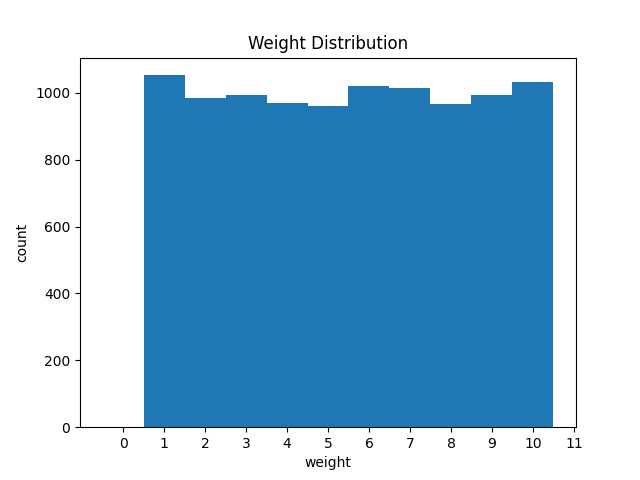
\includegraphics[width=\textwidth]{fig/asg1_weight_dist.png}
        \caption{Item weight distribution}
        \label{fig:weightdist}
    \end{subfigure}
    %\caption {}
    \label{fig:gain}
\end{figure*}

average result close to the expected optimal, scale the number of runs will change the number, but the result of the experiment is bigger, as plotted in figure \ref{fig:weightdist}, the reason might be the distribution of items weights not strictly align to 0.1 probability, more specifically, with seed 42, the average weight of items is 5.4972 
\subsection{Results}
\begin{figure}[htbp]
    \centering
    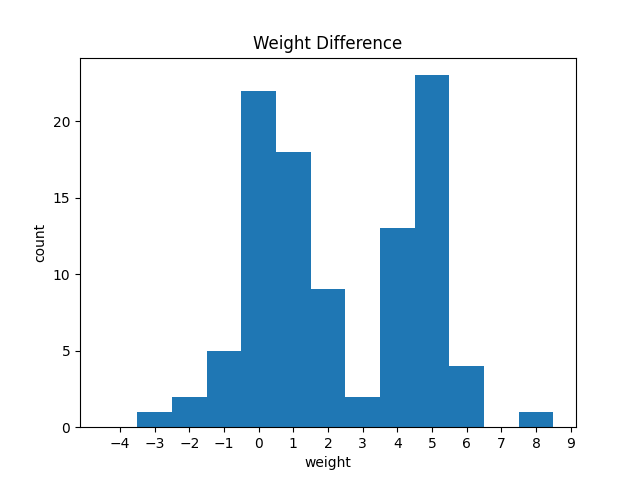
\includegraphics[width=0.8\linewidth]{fig/asg1_weight_diff.png}
    \caption {Remaining weights difference}
    \label{fig:gain}
\end{figure}



\subsection{Discussion}
\section{Conclusion}
In this report, we have %presented a thorough introduction to the design and underlying motivation of the two Evolutionary Algorithms (EAs). Through a comparative analysis of their performance in two distinct experiments, we have unveiled their strengths, potential drawbacks, and provided insights into when each EA is most suitable for a given scenario.
%\newpage
